\documentclass[a4paper,11pt]{article}
\usepackage[T1]{fontenc}
\usepackage[utf8]{inputenc}
\usepackage{lmodern}
\usepackage{graphicx}

\title{Neural network notes}
\author{Marco Marini}

\begin{document}

\maketitle
\tableofcontents

\begin{abstract}
Wall game
\end{abstract}

\section{General}

Wall is a game where a ball is moving in a rectangular field with diagonal trajectories

The upper and lateral bounds are constituted by wall that make the ball bouncing.
Indeed the bottom portion is open and a player controlled pad moves horizontally
allowing the player to bounce the ball inside the playing field.
The numbering of line starts from the bottom to upwards.

$
\begin{array}{ccccccccccccccc}
=	& = & = & = & = & = & = & = & = & = & = & = & = & = & = \\
|	&  &  &  &  &  &  &  &  &  &  &  &  &  & | \\ 
|	&  &  &  &  &  &  &  &  &  &  &  &  &  & | \\ 
|	&  &  &  &  &  &  &  &  &  &  &  &  &  & | \\ 
|	&  &  &  &  &  &  &  &  &  &  &  &  &  & | \\ 
|	&  &  &  &  &  &  &  &  &  &  &  &  &  & | \\ 
|	&  &  &  &  &  & O &  &  &  &  &  &  &  & | \\ 
|	&  &  &  &  &  &  &  &  &  &  &  &  &  & | \\ 
|	&  &  &  &  &  &  &  &  &  &  &  &  &  & | \\ 
|	&  &  &  &  &  &  &  &  &  &  &  &  &  & | \\ 
	&  &  & = & = & = &  &  &  &  &  &  &  &  & 
\end{array} 
$

Let it be
\[ n = 10 \] the row number
\[ m = 13 \] the column number
\[ w = 3 \] the pad width


\section{State space}

At any time the game state is represented by the position
of the ball, the direction of the ball and the position of pad.
We enumerate the possible states:

Pad may be located at one of \[m - w + 1 = 11 \] possible locations.

\subsection{Ball in the field}

When the ball is not located in the proximity of the walls or the pad
it can move in four different directions : NE, SE, SW, NW.

We have
\[ 4 (n-2)(m-2) (m - w + 1) = 3872 \]
possible states.

\subsection{Ball in upper corners}

In the upper corners the ball may have only one direction (NO in the west corner and NE in the east corner) then
you add more
\[
	2 (m - w +1) = 11
\] states.

\subsection{Ball in upper wall}

Instead when it is located in proximity of the upper wall it can have only two directions (NE or NW) then
\[
	( m - w + 1 ) 2 ( m - 2 ) = 242
\]
states.

\subsection{Ball in side wall}

When it is in proximity of the side wall, the ball can take only two possible directions (SE, NE if in the east side and SW, NW if in the west side), then we have
 \[ 2 (m - w + 1) 2 (n - 2) = 352 \]
additional states.


\section{Certain bounce}

We enumarate now how many states generate positive rewards regardless of strategy.

The pad is completely left, the ball can be completely left with only the NE possible direction, or it can be in the next two columns with directions NW or NE, or in fourth column with the direction NW
\[ 1 + 2(w-1) + 1 = 2w =  6 \]
possible states.

Symmetrically we have six other states when the racket is completely right.

The pad is located between the second column and fourth last column, the ball may be in the next three columns with NW or NE directions
\[
2w(m-w-2) = 48
\]
possible states.

we have totaly
\[
4w+2w(m-w-2) = 2w(m-w)=60
\]
possible states.


\section{End game}

We enumerate now how many states where, regardless of the strategy, you get to the end of game.

When the pad is in the first column and the ball is in fourth or fifth column with SE direction or between sixth and second last column with two possible directions or finally the ball is in last column with SW direction

\[
2(m-w-3)+3=2(m-w)-3=17
\]
possible states.

When the pad is located in the second column and the ball is located in the fifth or sixth column with SE direction or between the seventh and second last column with two possible directions or, finally, the ball is located in the last column with SW direction
\[
2(m-w-4)+3 = 2(m-w)-5 = 15
\]
possible states.

When the pad is located in the third column and the ball is located in the second column with SW direction or in sixth or seventh column with SE direction or between the eighth and the penultimate column with two possible directions or, finally, the ball is located in the last column with SW direction
\[
2(m-w-5)+4= 2(m-w)-6 = 14
\]
possible states.

We have the same states for symmetry when the pad is in the opposite side.

Quando la racchetta si trova tra la quarta colonna e sei colonne prima dell'ultima e la pallina si trova nei bordi con singole direzioni, o nelle due adiacenti la sx o la dx della racchetta con singole direzioni o nelle colonne intermedie tra i bordi e le precedenti colonne con due direzioni

When the pad is between the fourth column and six columns before the last and the ball is in the borders with single drections, or in the two adjacent left or right cells of the pad with single direction or intermediate columns between the edges and previous columns with two directions
\[
2(m-w-6)+6 = 2(m-w)-6=14
\]

We have in total
\[
\begin{array}{r}
 2[2(m-w)-3+2(m-w)-5+2(m-w)-6]+2(m-w)-6 = \\
 = 12(m-w)-28+2(m-w)-6 = \\
 = 14(m-w)-34 = 106 \\
\end{array}
\]
end game states.


\section{Conditional bounce}

We now states the bounces dependent by strategy.

When the pad is in the first column and the ball in the fifth column with SW direction
\[
1
\]
possible state.

Quando la racchetta si trova in seconda colonna e la pallina in prima colonna con direzione SE o in quinta o sesta colonna con direzione SW

When the pad is in the second column and the ball in the first column with the SE direction or fifth or sixth column with sw direction
\[
3
\]
possible states.

As many states by symmetry.

Quando la racchetta si trova tra la terza e cinque colonne prima dell'ultima, la pallina nelle due colonne antecedente la racchetta
con direzione SE o nelle duce colonne sucessiva la fine della racchetta
con direzione SW
When the pad is located between the third and five columns before the last, the ball in the two columns before the pad with 
SE direction or in the next two columns after the end of the pad
with SW direction
\[
4 (m-w-4)=4(m-w)-16=24
\]

We have totaly 
\[
(1+3)2+4(m-w)-16=4(m-w)-8=32
\]
possible states.


\section{Miglior policy}

The best policy is to bounce the ball once it reaches the bottom of the field

The ball bounces every
\[
2 (n - 1)
\]
steps.

The expected return after $ i = (1 \dots 2(n-1) $ steps from the bounce is 
\[
R_i = \gamma ^ {2(n-1)-i} \sum_{j=0}^{\infty} R^+ \gamma ^ {2(n-1)j} =
R^+ \frac{ \gamma ^ {2(n-1)-i}}{1-\gamma ^ {2(n-1)}}
\]


\section{Considerations}

Now consider the strategy $ \varepsilon $-greedy where a random action is generated with probability $ \varepsilon $.

Suppose the random action will lead to the end of the game.

What chance do we have that the sequence ends with the end of the game after $ k $ iterations?
\[
P(end) = 1 - (1 - \varepsilon) ^ k
\]
For an episodic sequence we have 
\[ k = 2 (n-1) \]
then
\[
P(end) = 1 - (1 - \varepsilon) ^ {2(n-1)}
\]

So if we want the end of the game happen with probability $ p $ we need 
\[
\varepsilon = 1- (1 - p) ^ \frac{1}{2(n-1)}
\]

E.g if $ p = 0.1 $ we have
\[
\varepsilon \approx 5.8363 \cdot 10^{-3}
\]

\section{Batch critic}

To enhance learning of critic component we can apply
the learning algorithm iteratively on a limited subset
of past experiences (SARS initial state, action, award, final state)
concurrently with the online learning algorithm.

The pictures (\ref{fig:seed1234}, \ref{fig:seed1234}, \ref{fig:seed31415}) represent the average length of the episodes in
the wall game in cases of purely on line algorithm  and
of in the batch one where interaction is delayed by 0, 200, 600 milliseconds
to allow the learning by different seeds of the random generator.

From the charts we can notice very different behaviors between the two algorithms.

In the first case (\ref{fig:seed1234}) we see that the two algorithms behave similarly when the reaction time is null.
While we notice an inertia to change when the reaction is delayed by 200 ms.

\begin{figure}
	\label{fig:seed1234}
	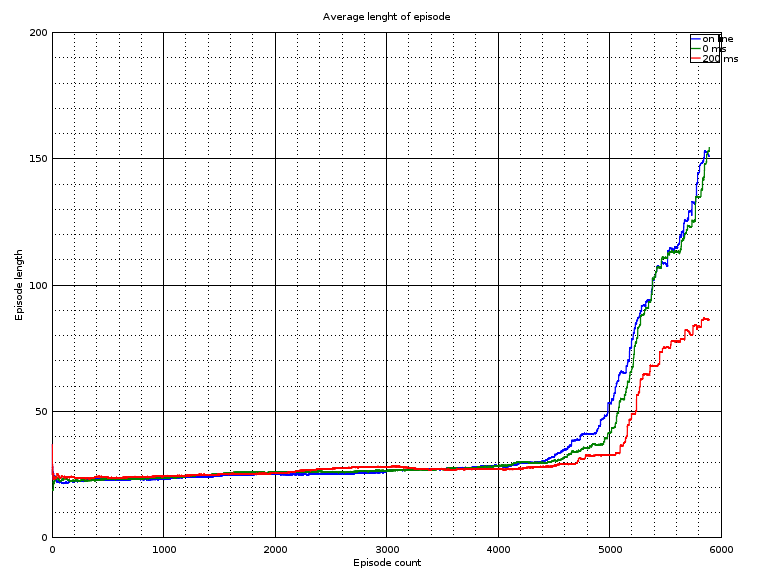
\includegraphics[width=300pt]{episodes-123}
	\caption{Seed 1234}
\end{figure}

In the second case (\ref{fig:seed4321}) however we note that the on-line algorithm has not found any best strategy.

\begin{figure}
	\label{fig:seed4321}
	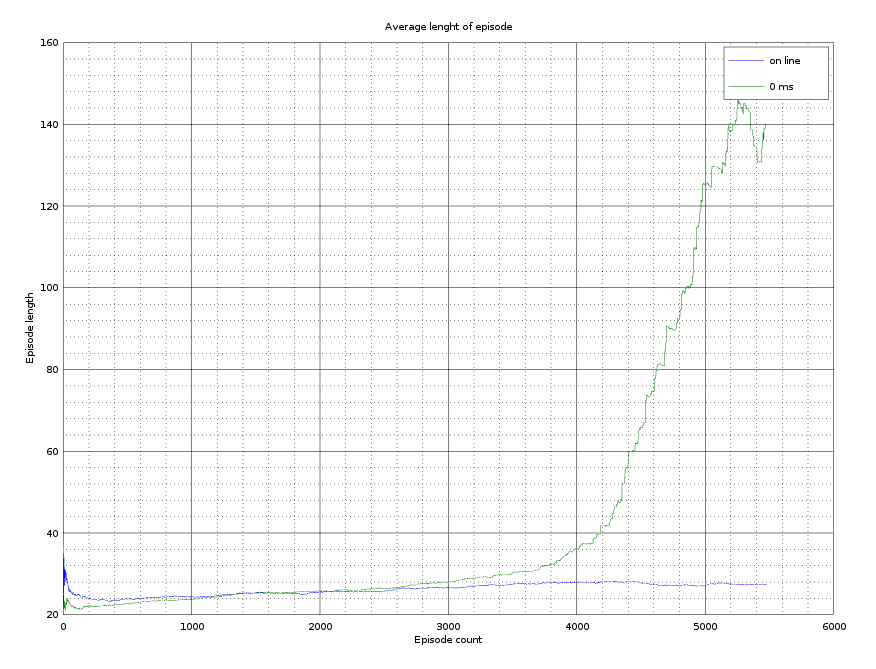
\includegraphics[width=300pt]{episodes-321}
	\caption{Seed 4321}
\end{figure}

In the third case (\ref{fig:seed31415}) the batch algorithm has found a better strategy before the on-line one.

\begin{figure}
	\label{fig:seed31415}
	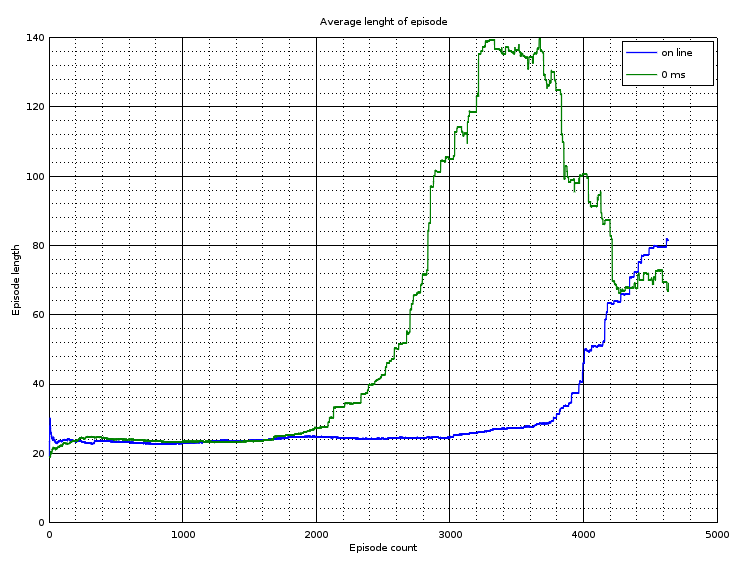
\includegraphics[width=300pt]{episodes-314}
	\caption{Seed 31415}
\end{figure}

Based on these evidences we can give the impression that the batch algorithm does not behave worse than online.

It would be interesting to better analyze these behaviors to search the general principles (eg speed of convergence of solutions or reactivity) from which the theories can be deduced.

\end{document}
